\begin{pastexam}[label={px:ccu-108-swa-01}]{中正資工所甲組 108 學年度 第 2 題}
（問答）

(8\%) To build a binary search tree, the following elements are inserted in the given order:
65, 50, 80, 70, 60, 62, 90, 10. You have to use the following struct \textit{treeNode} with one
additional filed \textit{leftSize}, where the field \textit{leftSize} of a tree node $u$ denotes
the number of tree nodes in the $u$'s left subtree plus one. For example, if the number of nodes
in the left subtree of the tree node $u$ is 3, then the tree node $u$'s field \textit{leftSize} is
equal to 4.
\begin{enumerate}[label=(\alph*)]
\item (3\%) Please draw the binary search tree, and each tree node stores its element and
\textit{leftSize}.
\item (5\%) Please illustrate how to obtain the tree node storing the $k$-th smallest element in
the binary search tree built in (a) from the tree root, and explain your procedure. Note that you
have to use the additional field \textit{leftSize} and the time complexity of your procedure
should be $O(\log n)$, where $n$ is the number of input elements.
\end{enumerate}
\begin{code}{c}{原題的結構}
typedef struct _tree_node_ *treePointer;
typedef struct _tree_node_ {
    treePointer leftChild;
    treePointer rightChild;
    int element;
    int leftSize;
} treeNode;
\end{code}
\end{pastexam}

\begin{pastsoln}
\textbf{(a)} 依序插入（資結書第~9.2~節）：$65$ 當根；$50 < 65$ 往左；$80 > 65$ 往右；$70$ 在 $65$
右邊、$80$ 左邊；$60$ 在 $65$ 左邊、$50$ 右邊；$62$ 再往下到 $60$ 的右邊；$90$ 在 $80$ 右邊；
$10$ 在 $50$ 左邊。 下圖節點右上方的小字是 \textit{leftSize}（左子樹節點數加 $1$）。 例如根
$65$ 的左子樹 $\{50, 10, 60, 62\}$ 有 $4$ 個節點，\textit{leftSize} 是 $5$；$60$ 沒有左子樹，是
$1$。

\begin{center}
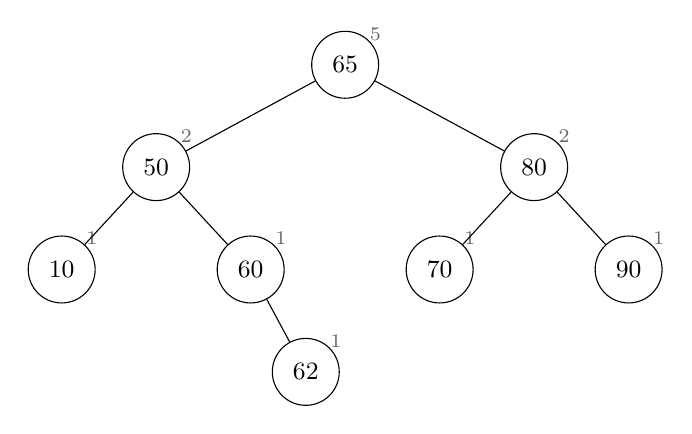
\begin{tikzpicture}[
    every node/.style={circle, draw, minimum size=8.5mm, inner sep=0pt, font=\small},
    ls/.style={draw=none, rectangle, minimum size=0pt, font=\scriptsize, text=black!60},
    level distance=13mm,
    level 1/.style={sibling distance=48mm},
    level 2/.style={sibling distance=24mm}, level 3/.style={sibling distance=14mm}]
\node[label={[ls]45:5}] {65}
  child {node[label={[ls]45:2}] {50}
    child {node[label={[ls]45:1}] {10}}
    child {node[label={[ls]45:1}] {60}
      child[missing]
      child {node[label={[ls]45:1}] {62}}}}
  child {node[label={[ls]45:2}] {80}
    child {node[label={[ls]45:1}] {70}}
    child {node[label={[ls]45:1}] {90}}};
\end{tikzpicture}
\end{center}

\textbf{(b)} \textit{leftSize} 就是資結書第~9.4~節的 $r = x.\mathit{left}.\mathit{size} + 1$：節點在
自己這棵子樹裡排第幾小。 從根開始，比較 $k$ 和 \textit{leftSize}：
\begin{itemize}
\item $k = \textit{leftSize}$：這個節點就是答案。
\item $k < \textit{leftSize}$：答案在左子樹，仍然找第 $k$ 小。
\item $k > \textit{leftSize}$：左子樹和這個節點共 \textit{leftSize} 個都比答案小，到右子樹找第
$k - \textit{leftSize}$ 小。
\end{itemize}
這就是資結書虛擬碼~9.8 的 \proc{Tree-Select}，寫成題目的結構：

\begin{code}{c}{第 $k$ 小（$k$ 從 $1$ 開始）}
treePointer kth_smallest(treePointer t, int k)
{
    while (t != NULL) {
        if (k == t->leftSize)
            return t;
        if (k < t->leftSize) {
            t = t->leftChild;
        } else {
            k -= t->leftSize;
            t = t->rightChild;
        }
    }
    return NULL;            // k < 1 或 k 大於節點數
}
\end{code}

例子：找第 $6$ 小。

\begin{center}
\begin{tabular}{ccccl}
\toprule
步 & 節點 & $k$ & \textit{leftSize} & 動作 \\
\midrule
1 & 65 & 6 & 5 & $k > 5$，$k \gets 6 - 5 = 1$，往右 \\
2 & 80 & 1 & 2 & $k < 2$，往左 \\
3 & 70 & 1 & 1 & 相等，回傳 $70$ \\
\bottomrule
\end{tabular}
\end{center}

由小到大是 $10, 50, 60, 62, 65, 70, 80, 90$，第 $6$ 小確實是 $70$。 再舉一個往左的例子，第 $4$ 小：
$65$（$4 < 5$，往左）、$50$（$4 > 2$，$k \gets 2$，往右）、$60$（$2 > 1$，$k \gets 1$，往右）、
$62$（相等），回傳 $62$。

\textbf{正確性}：迴圈維持「答案是目前子樹裡第 $k$ 小」。 三種情況都保持這件事：相等時目前節點
前面恰好有 $k - 1$ 個較小的數；往左時答案的排名不變；往右時跳過的 \textit{leftSize} 個數都比
右子樹的數小，排名減去 \textit{leftSize}。

\textbf{複雜度}：每一步往下一層，最多走 $h$ 步（$h$ 是樹高），每步 $O(1)$，時間 $O(h)$。 題目
要求 $O(\log n)$：這棵樹的 $h = 4$；一般的 BST 只有在高度是 $O(\log n)$ 時才成立（例如資結書
第~10~章的平衡樹，或隨機插入時的期望情況，資結書第~9.3~節），依序插入由小到大的數時 $h = n$，
時間是 $\Theta(n)$。 作答時把「$O(h)$，平衡時為 $O(\log n)$」寫清楚。 另外，插入或刪除時，
路徑上每個「往左走」的節點的 \textit{leftSize} 要加 $1$ 或減 $1$，才能一直保持正確。
\end{pastsoln}
